\documentclass[12pt]{article}
\usepackage[a4paper, portrait, margin=1cm, right=1cm]{geometry}
\usepackage{fontspec}
\usepackage[fleqn]{amsmath}
\usepackage{setspace}
\usepackage{graphicx}
\usepackage{amssymb}

\graphicspath{./graphics/}
\setmainfont[Ligatures=TeX]{Linux Libertine}

\DeclareMathOperator{\arcctg}{arcctg}
\DeclareMathOperator{\const}{\textit{const}}
\DeclareMathOperator{\rank}{rank}

\title{АиГ. Подготовка к экзамену}
\author{Студент группы 2305 Александр Макурин}
\date{16 января 2022}

\begin{document}
\newcommand{\limx}{\displaystyle\lim_{x \rightarrow x_0}}
\newcommand{\overo}{\overline{o}}
\newcommand{\ol}[1]{\overrightarrow{#1}}

\maketitle

\begin{sloppypar}
    \setstretch{1.8}

    Все случаи обозначеия векторов в формулах предполагают, что эти векторы ненулевые.

    \section{Определение, геометрическая интерпретация комплексных чисел в алгебраической форме. Сложение, вычитание, умножение, деление, возведение в степень комплексных чисел в алгебраической форме.}
    Комлексное число — выражение вида $a + bi$, где $a \in \mathbf{R}$ называют вещественной частью, а $b \in \mathbf{R}$ мнимой частью комлексного числа. $i$ - спецсимвол (корень из $-1$).
    Геометрически комплексное число есть точка в декартовой системе координат, где $a$ - это значение по оси абсцисс, а $b$ - значение по оси ординат.
    \begin{align*}
         & (a + bi) \pm (c + di) = (a \pm c) + (b \pm d)i                                                                                 \\
         & (a + bi) \cdot (c + di) = (ac - bd) + (ad + bc)i                                                                               \\
         & \dfrac{a + bi}{c + di} = \dfrac{(a + bi) \cdot (c - di)}{(c + di) \cdot (c - di)} = \dfrac{(ac + bd) + (cbi - adi)}{c^2 + d^2} \\
         & (a + bi)^n = (a + bi) \cdot (a + bi) \cdot ... \cdot (a + bi) \ \  \text{(n раз)}
    \end{align*}
    Если $z = a + bi$, то $\overline{z} = a - bi$ называют сопряжённым к числу $z$.
    Пример:
    \[
        (2 - 3i)^2 = 4 - 12i - 9 = -5 - 12i
    \]
    \section{Квадратные корни из комплексных чисел в алгебраической форме. Квадратные уравнения с комплексными коэффициентами и корнями в алгебраической форме.}
    Квадратными корнями комплексного числа $z = a + bi$ называют такие числа $z_1$ и $z_2$, что $z_1^2 = z$ и $z_2^2 = z$. Для нахождения квадратного корня комплексного числа используется уравнение вида $(c + di)^2 = a + bi$ ($a, b, c, d \in \mathbf{R}$), которое удобно представить как систему из двух уравнений:
    \[
        \begin{cases}
            c^2 - d^2 = a \\
            2cd = b
        \end{cases}
    \]
    Решением данной системы будут пары чисел $c$ и $d$, являющиеся вещественной и мнимой частью искомых корней соответственно.

    Решение уравнений с комплексными корнями требует знания того, что $\sqrt{-x} = i\sqrt{x}$. В остальном решение совпадает со стандартным решением квадратных уравнений. Решение уравнений вида $ax^2 + bx + c = 0$, где $a, b, c$ - комплексные числа происходит по стандартному алгоритму, но с вычислением корней из комплексных чисел:
    \begin{align*}
         & ax^2 + bx + c = 0                             \\
         & x_{1,2} = \dfrac{-b \pm \sqrt{b^2 - 4ac}}{2a}
    \end{align*}
    Пример (этот пример лютая дичь, лучше взять что-то вроде нахождения квадратного корня из чего-то типа $3 - 4i$):
    \begin{align*}
         & (4 + i)x^2 + (2 + i)x - 3 - 4i = 0                                                                                                    \\
         & x_{1,2} = \dfrac{-2 - i \pm \sqrt{3 + 4i - 4(4 + i)(-3 - 4i)}}{8 + 2i} = \dfrac{-2 - i \pm \sqrt{5}\sqrt{7 + 16i}}{8 + 2i}            \\
         & \left.\begin{cases}
                     a^2 - b^2 = 7 \\
                     2ab = 16
                 \end{cases}\right|
        \Rightarrow b = \dfrac{8}{a} \Rightarrow \dfrac{a^4 - 64}{a^2} = 7 \Rightarrow a^4 - 7a^2 - 64 = 0                                       \\
         & a^2 = \dfrac{7 \pm \sqrt{49 + 256}}{2} \Rightarrow a = \pm\sqrt{\dfrac{7 + \sqrt{305}}{2}}; b = \pm 8\sqrt{\dfrac{2}{7 + \sqrt{305}}} \\
         & x_{1,2} = \dfrac{(-2 - i \pm \sqrt{5}\left(\sqrt{\dfrac{7 + \sqrt{305}}{2}} + 8\sqrt{\dfrac{2}{7 + \sqrt{305}}}i\right))(8 - 2i)}{68}
    \end{align*}

    \section{Модуль и аргумент комплексного числа. Тригонометрическая форма комплексного числа. Умножение и возведение в степень комплексных чисел в тригонометрической форме.}
    Тригонометрическая форма комплексного числа: $z = r(\cos \varphi i\sin \varphi)$, где $z$ - комплексное число, $r$ - модуль комплексного числа (всегда $\ge 0$), $\varphi$ - аргумент комплексного числа (наклон прямой, проведённой в комплексной плоскости из начала координат в точку этого комплексного числа).

    Умножение и возведение в степень комплексных чисел в тригонометрической форме (сумма выводится через тригонометрические формулы $\cos(a + b)$ и $\sin(a + b)$, произведение через сумму):
    \begin{align*}
         & z_1 \cdot z_2 = r_1(\cos \varphi_1 + i \sin \varphi_1) \cdot r_2(\cos \varphi_2 i \sin \varphi_2) = r_1r_2(\cos(\varphi_1 + \varphi_2) + i \sin(\varphi_1 + \varphi_2)) \\
         & z^n = r^n(\cos n\varphi + i \sin n\varphi),\ n \in \mathbf{N}
    \end{align*}

    \section{Корни из комплексных чисел в тригонометрической форме.}
    \[
        \left.\begin{cases}
            z = r(\cos \varphi + i \sin \varphi) \\
            (p(\cos \beta + i \sin \beta))^n = z
        \end{cases}\right|
        \Rightarrow
        \begin{cases}
            p = \sqrt[n]{r} \\
            \cos n\beta = \cos \varphi \Rightarrow n\beta = \varphi + 2\pi k \Rightarrow \beta = \dfrac{\varphi}{n} + \dfrac{2\pi k}{n}, \ k=0, 1, 2, 3, ..., n-1
        \end{cases}
    \]
    При $k = n, \ \beta_0 = \beta_n$

    Пример:
    \[
        \sqrt{4(\cos \pi + i \sin \pi)} = 2(\cos{(\dfrac{\pi}{2} + \pi k)} + i\sin{(\dfrac{\pi}{2} + \pi k)}), \  k = 0, 1
    \]

    \section{Многочлены и действия над ними. Рациональные корни многочлена с целыми коэффициентами.}
    Многочлен порядка $n$ - выражение вида $\sum^n_{i = 0}(a_i x^i),\ a_n \neq 0$.

    Многочлены можно умножать, делить с остатком и складывать.
    Разделить многочлен $f(x)$ на многочлен $g(x)$ означает найти такие $q(x)$ и $r(x)$, что $f(x) = g(x)q(x) + r(x)$, при этом порядок $r(x)$ меньше, чем порядок $g(x)$.

    Если многочлен имеет целые коэффициенты и $\dfrac{p}{q}$ - рациональный корень (несократимая дробь), то
    \[
        \begin{cases}
            a_0\ \vdots\ p \\
            a_n\ \vdots\ q
        \end{cases}
    \]
    Доказательство:
    \begin{align*}
         & a_0 + a_1(\dfrac{p}{q}) + a_2(\dfrac{p}{q})^2 + ... + a_n (\dfrac{p}{q})^n = 0                                             \\
         & a_1(\dfrac{p}{q}) + a_2(\dfrac{p}{q})^2 + ... + a_n (\dfrac{p}{q})^n = -a_0 \ \ \ \ |\cdot q^n                             \\
         & a_1pq^n + a_2p^2q^{n - 1} + ... + a_n p^n = -a_0q^n                                                                        \\
         & \text{(Левая часть кратна $p$ $\Rightarrow$ правая кратна $p$), $\dfrac{p}{q}$ несократима $\Rightarrow$ $a_0$ кратно $p$} \\
         & \text{Аналогично $a_n$ кратно $q$}
    \end{align*}
    Пример:
    \begin{align*}
         & 1 - 3x + 2x^2 = 0      \\
         & p \in \{-1, 1\}        \\
         & q \in \{-2, -1, 1, 2\} \\
         & x_1 = 1                \\
         & 2x - 1 = 0             \\
         & x_2 =  \dfrac{1}{2}
    \end{align*}

    \section{Разложение многочленов на множители. Основная теорема алгебры. Следствие.}
    Основная теорема алгебры: «Каждый многочлен, не равный константе, имеет хотя бы один комплексный корень».
    Следствие: количество комплексных корней многочлена равно его степени, с учётом кратности корней.

    Из следствия основной теоремы алгебры следует, что любой многочлен можно разложить на множители степени 1:

    $f(z) = a_0(z - z_0)(z - z_1)...(z - z_{n-1})(z - z_n)$, где $z_{0..n}$ - корни многочлена $f(z)$, $a_0$ - коэффициент при старшем члене

    Пример:
    \[
        2x^2 - 3x + 1 = (x - 1)(2x - 1)
    \]

    \section{Приближенное вычисление корней многочленов. Разложение многочлена с вещественными коэффициентами на множители степени не выше 2. Теорема Виета для многочленов степени выше второй.}
    Приближенное вычисление корней многочлена может быть выполнено, к примеру, с помощью метода Ньютона: $x_{n + 1} = x_n - \dfrac{f(x_n)}{f'(x_n)}$, где $x_n$ - корень итерации $n$, $x_{n + 1}$ - корень следующей итерации (более высокой точности).

    Многочлен с вещественными коэффициентами может быть разложен на множители степени не выше 2. Множителями первой степени будут выражения с вещественными корнями, а а множители со степенью 2 будут получены в результате перемножения сопряжённых комплексных корней. Это следует из свойства, что если $z$ - комплексный корень, то $\overline{z}$ (сопряжённое к $z$) тоже является корнем.
    Доказательство:
    \begin{align*}
         & \text{Пусть } \exists z_1 = a + bi, z_2 = c + di \text{ - комплексные числа. Тогда:}                                                                                  \\
         & z_1 + z_2 = (a + c) + (b + d)i                                                                                                                                        \\
         & \overline{z_1 + z_2} = (a + c) - (b + d)i                                                                                                                             \\
         & \overline{z_1} + \overline{z_2} = a - bi + c - di = (a + c) - (b + d)i = \overline{z_1 + z_2}                                                                         \\
         & \overline{z_1 \cdot z_2} = (ac - bd) - (cb + ad)i                                                                                                                     \\
         & \overline{z_1} \cdot \overline{z_2} = (a - bi)(c - di) = (ac - bd) - (cb + ad)i                                                                                       \\
         & \text{Отсюда: } \overline{z^n} = \overline{z}^n \text{ (легко доказывается через мат. индукцию)}                                                                      \\
         & \text{Соответсвенно: } \sum_{i = 0}^n a_i x^i = 0 \Rightarrow \overline{\sum_{i = 0}^n a_i x^i} = \overline{0} = 0 \Rightarrow{\sum_{i = 0}^n a_i \overline{x}^i = 0}
    \end{align*}

    Теорема Виета для многочленов степени выше второй:

    Пусть старший коэффициент многочлена = 1, тогда многочлен будет представлять собой $x^n + a_{1}x^{n - 1} + ... + a_{n-1}x + a_n$. При этом справедливы следующие равенства:
    \[
        \begin{array}{ll}
            a_{1}\cdot(-1)^{1} & = x_1 + x_2 + ... x_n                                                                           \\
            a_{2}\cdot(-1)^{2} & = x_1x_2 + x_1x_3 + x_1x_4 + ... + x_1x_n + x_2x_3 + x_2x_4 + ... + x_2x_n + ... + x_{n - 1}x_n \\
                               & \vdots                                                                                          \\
            a_{n}\cdot(-1)^{n} & = x_1x_2x_3 ... x_{n-1}x_n                                                                      \\
        \end{array}
    \]

    Пример:
    \begin{align*}
         & f(x) = x^2                                     \\
         & x_0 = 100                                      \\
         & x_1 = 100 - \dfrac{10000}{200} = 100 - 50 = 50 \\
         & x_2 = 50 - \dfrac{2500}{100} = 50 - 25 = 25    \\
         & x_3 = 25 - \dfrac{625}{50} = 12.5              \\
         & x_4 = 12.5 - \dfrac{156.25}{25} = 6.25         \\
         & ...
    \end{align*}

    \section{Дробно-рациональные функции. Разложение правильной дроби на простейшие.}
    Дробно-рациональной функцией (дробью) называется выражение вида $\dfrac{f(x)}{g(x)}$, где $f(x)$ и $g(x)$ - многочлены. Если порядок $f(x)$ строго меньше порядка $g(x)$, то такая дробь называется правильной.

    Для разложения правильной дроби на простейшие нужно записать её в виде суммы простейших дробей с неопределёнными коэффициентами, где в знаменателях все возможные множители знаменателя начальной дроби.
    Для нахождения неопределённых коэффициентов нужно привести к общему знаменателю все простейшие дроби и приравнять результат к начальной дроби. Затем найти коэффициенты либо подстановкой $x$-ов (удобнее всего подставлять корни многочлена-знаменателя), либо составить систему уравнений, приравнивая коэффициенты при равных степенях у левого и правого числителей.

    Пример:
    \[
        \begin{array}{l}
            \dfrac{1}{x^2 - 5x + 6} = \dfrac{1}{(x-2)(x+3)} = \dfrac{a}{x - 2} + \dfrac{b}{x-3} = \dfrac{a(x - 3) + b(x-2)}{x^2 - 5x + 6} = \dfrac{(a + b)x - 3a - 2b}{x^2 - 5x + 6} \\
            \Rightarrow \left.\begin{cases}
                                  a + b = 0 \\
                                  -(3a + 2b) = 1
                              \end{cases}\right|
            \Rightarrow a = -1; b = 1                                                                                                                                                \\
            \dfrac{1}{x^2 - 5x + 6} = \dfrac{-1}{x - 2} + \dfrac{1}{x - 3}                                                                                                           \\
        \end{array}
    \]

    \section{Матрицы и основные действия над ними (сложение, вычитание, умножение матрицы на число, умножение матриц).}
    Матрица - прямоугольная таблица чисел, функций или алгебраических выражений, состоящая из строк одинаковой длины. Если количество строк и столбцов совпадает, то такая матрица зовётся квадратной матрицей порядка $n$, где $n$ - количество строк/столбцов в матрице. $A_{n\times m}$ - матрица, содержащая $n$ строк и $m$ столбцов. $n \times m$ - размер матрицы
    \[
        A = \begin{pmatrix}
            a_{11} & a_{12} & a_{13} \\
            a_{21} & a_{22} & a_{23} \\
            a_{31} & a_{32} & a_{33} \\
        \end{pmatrix}
        \text{ - квадратная матрица 3-го порядка}
    \]

    В общем виде матрица может быть записана как $A = \left(a_{ij}\right)$, где $a_{ij}$ - элемент матрицы, находящийся на пересечении строки $i$ и столбца $j$.

    Пусть $A = \left(a_{ij}\right)$ и $B = \left(b_{ij}\right)$ - матрицы одинакового размера, $c$ - константа. Тогда:
    \begin{align*}
         & A \pm B = \left(a_{ij} \pm b_{ij}\right)         \\
         & c\cdot A = A\cdot c = \left(c\cdot a_{ij}\right)
    \end{align*}

    Пусть $A_{n \times k}, \ B_{k \times m}$. Тогда:
    \[
        A \times B = \left(\sum^k_{l=1} a_{il}b_{lj}\right) = C_{n \times m} \neq B \times A
    \]
    Умножение матриц не коммутативно.

    Пример:
    \[
        \begin{pmatrix}
            1 & 2 & 3 \\
            4 & 5 & 6 \\
        \end{pmatrix}
        +
        \begin{pmatrix}
            9 & 8 & 7 \\
            6 & 5 & 4 \\
        \end{pmatrix}
        =
        \begin{pmatrix}
            10 & 10 & 10 \\
            10 & 10 & 10 \\
        \end{pmatrix}
    \]

    \section{Возведение матрицы в степень. «Квадратный корень» из матрицы. Значение многочлена от матрицы. Геометрический смысл сложения и умножения матриц.}
    Возведение матрицы $A$ в степень $n$ есть ничто иное, как $A \cdot A \cdot ... \cdot A$ ($n$ множителей). При этом очевидно, что умножать можно только квадратные матрицы.

    Квадратный корень из матрицы $A$ - задача по нахождению такой матрицы $B$, что $B^2 = A$. Может быть решена посредством составления матрицы $B$ из неопределённых коэффициентов и решения системы линейных уравнений. Количество ответов бесконечно, если порядок матрицы больше 1. Применимо только к квадратным матрицам.

    Многочленом $f(x)$ от квадратной матрицы $A$ является тот же многочлен $f(x)$ с подстановкой $A$ в качестве $x$ и заменой одночлена $a_n$ нулевого порядка на $a_nE$, где $E$ - единичная матрица того же порядка, что и $A$.

    Линейное преобразование пространства можно представить в виде матрицы. Геометрический смысл сложения матриц - сложение преобразований, умножения матриц - композиция преобразований (последовательное применение).

    Пример:
    \[
        \begin{pmatrix}
            1 & 2 \\
            3 & 4 \\
        \end{pmatrix}^2
        =
        \begin{pmatrix}
            7  & 10 \\
            15 & 22 \\
        \end{pmatrix}
    \]

    \section{Определитель матрицы второго и третьего порядка. Свойства определителей второго порядка.}
    Определителем матрицы второго порядка $A = \begin{pmatrix}
            a_{11} & a_{12} \\
            a_{21} & a_{22} \\
        \end{pmatrix}$ называют число $a_{11}a_{22} - a_{12}a_{21}$. Обозначение: $\det A$ или $\begin{vmatrix}
            a_{11} & a_{12} \\
            a_{21} & a_{22} \\
        \end{vmatrix}$.

    Определителем матрицы третьего порядка $A = \begin{pmatrix}
            a_{11} & a_{12} & a_{13} \\
            a_{21} & a_{22} & a_{23} \\
            a_{31} & a_{32} & a_{33} \\
        \end{pmatrix}$ называют число $a_{11}a_{22}a_{33} - a_{11}a_{23}a_{32} + a_{12}a_{23}a_{31} - a_{12}a_{21}a_{33} + a_{13}a_{21}a_{32} - a_{13}a_{22}a_{31}$

    Свойства определителей второго порядка:
    \begin{itemize}
        \item $\det A = \det {A^T}$
        \item Определитель матрицы равен определителю этой же матрицы с переставленными строками или столбцами, умноженному на -1.
        \item Если одну строку или столбец домножить на $k$, то определитель матрицы измениться в $k$ раз.
        \item Если строки или столбцы равны, то определитель матрицы равен 0.
        \item Произведение определителей двух матриц равно определителю произведения этих матриц.
    \end{itemize}


    Пример:
    \[
        \begin{vmatrix}
            1 & 2 \\
            3 & 4 \\
        \end{vmatrix} = 4 - 6 = -2
    \]

    \section{Определение определителя матрицы порядка n. Чётные и нечетные перестановки.}
    Перестановкой набора чисел $(n_1, n_2, n_3)$ называется запись этих же чисел в другом порядке. Когда количество неправильных пар в перестановке чётное, перестановка называется чётной, иначе - нечётной. Неправильная пара - случай, когда в наборе чисел меньшее число идёт после большего.

    Определитем матрицы порядка $n$ называется сумма произведений элементов матрицы, номером столбца которых будут элементы перестановок, на -1 в степени чётности этих перестановок:
    \[
        \det A = \sum_{k_1, k_2, ..., k_n}(-1)^{t(k_1,k_2,...,k_n)}a_{1k_1}a_{2k_2}a_{3k_3}...a_{nk_n}
    \]
    Где рассматривают все варианты перестановки $(k_1, k_2, ..., k_n)$, а $t(k_1,k_2,...,k_n)$ - чётность перестановки.

    Пример:
    \[
        \begin{vmatrix}
            1 & 2 \\
            3 & 4 \\
        \end{vmatrix} = 1 \cdot 4 \cdot (-1)^0 + 2 \cdot 3 \cdot (-1)^1 = -2
    \]

    \section{Вычисление определителей произвольного порядка (три способа).}
    \begin{itemize}
        \item Через чётности перестановок: $\displaystyle \det A_{n \times n} = \sum_{k_1, k_2, ..., k_n} (-1)^{t(k_1, k_2, ..., k_n)}a_{1k_1}a_{2k_2}...a_{nk_n}$, $t(k_1, k_2, ..., k_n)$ - чётность перестановки.
        \item Через разложение по строке/столбцу - определителем матрицы будет сумма произведений элементов $a_{ij}$ этой строки/столбца на $(-1)^{i + j}$ на определитель матрицы, полученной из исходной посредством вычёркивания строки $i$ и столбцы $j$.
        \item Через элементарные преобразования и приведение к верхнему/нижниму диагональному виду — тогда определитель матрицы будет равен произведению элементов на главной диагонали (определитель при элементарных преобразованиях не меняется).
        \item С помощью Конденсации Доджсона: \begin{itemize}
                  \item 1. С помощью элементарных преобразований делаем внутренние элементы матрицы $A_{n\times n}$ не равными 0 ($a_{ij} \neq 0,\ \ i,j \notin \{1, n\}$)
                  \item 2. Строим матрицу $B_{(n - 1) \times (n - 1)}$ из миноров матрицы $A$: $b_{ij} = \begin{vmatrix}
                                a_{ij}       & a_{i, j+ 1}     \\
                                a_{i + 1, j} & a_{i + 1, j+ 1} \\
                            \end{vmatrix}$
                  \item 3. Строим матрицу $C{(n - 2) \times (n - 2)}$, разделив миноры матрицы $B$ на внутренние элементы матрицы $A$: $c_{ij} = \dfrac{\begin{vmatrix}
                                    b_{ij}       & b_{i, j + 1}     \\
                                    b_{i + 1, j} & b_{i + 1, j + 1} \\
                                \end{vmatrix}}{a_{i + 1, j + 1}}$
                  \item 4. Пусть $A=B$ и $B=C$. Повторяем шаг 3, пока не придём к матрице первого порядка - её единственный элемент и будет ответом.
              \end{itemize}
    \end{itemize}
    Пример:
    \[
        \begin{vmatrix}
            1 & 2 \\
            3 & 4 \\
        \end{vmatrix} = 1 \cdot 4 \cdot (-1)^0 + 2 \cdot 3 \cdot (-1)^1 = -2
    \]


    \section{Обратная матрица. Определение, свойства. Вычисление обратной матрицы (два способа).}
    Обратной матрицей к квадратной матрице $A$ называется такая матрица $A^{-1}$, что $AA^{-1} = A^{-1}A = E$.
    Свойства обратной матрицы:
    \begin{itemize}
        \item $(aA)^{-1} = a^{-1}A^{-1}$, $a \neq 0$
        \item $(AB)^{-1} = B^{-1}A^{-1}$
        \item $(A^{-1})^T = (A^T)^{-1}$
    \end{itemize}
    Вычисление обратной матрицы:
    \begin{itemize}
        \item Способ 1. Обозначим $A^{(i, j)}$ - матрица, полученная в результате вычёркивания столбца $j$ и строки $i$ из матрицы $A$. $A^*$ - результат транспонирования матрицы, составленной из выражений вида $(-1)^{i + j}A^{(i, j)}$. Тогда $A^{-1} = \dfrac{A^*}{\det A}$, если $\det A \neq 0$.
        \item Способ 2. Припишем к матрице $A_{n \times n}$ справа единичную матрицу порядка $n$. Затем с помощью элементарных преобразований сведём левую часть (изначально $A$) получившейся матрицы к единичной. Тогда матрица, получившаяся справа и будет искомой обратной матрицей: $(A|E) \rightarrow (E|A^{-1})$.
    \end{itemize}

    Пример:
    \[
        \begin{pmatrix}
            1 & 2 \\
            3 & 4 \\
        \end{pmatrix}
        \Rightarrow
        \left(\begin{array}{ll|ll}
                1 & 2 & 1 & 0 \\
                3 & 4 & 0 & 1 \\
            \end{array}\right)
        \sim
        \left(\begin{array}{rr|rr}
                1 & 2  & 1  & 0 \\
                0 & -2 & -3 & 1 \\
            \end{array}\right)
        \sim
        \left(\begin{array}{rr|rr}
                1 & 0 & -2  & 1    \\
                0 & 1 & 3/2 & -1/2 \\
            \end{array}\right)
        \Rightarrow
        \begin{pmatrix}
            1 & 2 \\
            3 & 4 \\
        \end{pmatrix}^{-1}
        =
        \begin{pmatrix}
            -2  & 1    \\
            3/2 & -1/2 \\
        \end{pmatrix}
    \]

    \section{Арифметические векторы. Ранг матрицы. Признаки линейно зависимой системы.}
    Вектор - матрица, у которой ширина либо высота равна 1. Ранг матрицы - ранг (размерность) линейной оболочки этой матрицы. Система арифметических векторов $\Vec{x_1}, \Vec{x_2}, ..., \Vec{x_n}$ является линейно зависимой если существует такой набор $a_1, a_2, ..., a_n$, содержащий хотя бы один ненулевой элемент, что $\sum_{i = 1}^n \Vec{x_i}a_i = 0$. Иначе система линейно независима.

    Признаки линейно зависимой системы:
    \begin{itemize}
        \item Есть 2 равных вектора
        \item Есть пара векторов, таких что $\Vec{x_i} = k\Vec{x_j}$ ($k \in R$)
        \item Есть нулевой вектор
        \item Есть линейно зависимая подсистема
    \end{itemize}

    Пример:
    \[
        \Vec{x_1} = (0, 1, 2); \Vec{x_2} = (3, 4, 5) \Rightarrow \Vec{x_1} + \Vec{x_2} = (3, 5, 7)
    \]

    \section{Методы вычисления ранга матрицы (три способа).}
    Ранг матрицы не меняется в результате элементарных преобразований.

    \begin{itemize}
        \item Метод элементарных преобразований (Гаусса). Ранг матрицы равен количеству количеству строк после приведения её к верхнетреугольному виду, содержащих ненулевой элемент на главной диагонали. Другими словами, ранг матрицы равен количеству линейно независимых строк этой матрицы.
        \item Определитель квадратной матрицы. Если определитель матрицы $\neq$ 0, то её ранг равен её размеру. Иначе ранг < размера.
        \item Метод окаймляющих миноров. Минор матрицы $A$ - определитель квадратной матрицы $B$, полученной в результате вычеркивания некоторого количества строк и столбцов из матрицы $A$. Если минор = 0, то он называется вырожденным, иначе - невырожденным. Ранг матрицы равен размеру самого большого невырожденного минора, такого, что все миноры большего размера, чьи матрицы содержат матрицу этого минора, вырождены.
    \end{itemize}

    \[
        \rank \begin{pmatrix}
            1 & 2 & 3 \\
            2 & 4 & 6 \\
            4 & 5 & 6 \\
        \end{pmatrix} = \rank \begin{pmatrix}
            1 & 2  & 3  \\
            0 & -3 & -6 \\
            0 & 0  & 0  \\
        \end{pmatrix} = 2
    \]

    \section{Системы линейных уравнений. Правило Крамера.}
    Системой линейных уравнений называют систему уравнений вида $\sum^m_{i = 1}a_{ki}x_i = b_k$, где $k = 1, 1, 2, ..., n$ - номер строки уравнения, $a_{ki}$ - коэффициент при $x_i$ в строке $k$, а $b_k$ - правая часть уравнения в строке $k$.

    Также можно записать такую систему в виде $AX = B$, где:
    \begin{alignat*}{2}
        A = \begin{pmatrix}
                a_{11} & a_{12} & \dots  & a_{1m} \\
                a_{21} & a_{22} & \dots  & a_{2m} \\
                \vdots & \vdots & \ddots & \vdots \\
                a_{n1} & a_{n2} & \dots  & a_{nm}
            \end{pmatrix};\  &
        B = \begin{pmatrix}
                b_1    \\
                b_2    \\
                \vdots \\
                b_n
            \end{pmatrix};\                   &
        X = \begin{pmatrix}
                x_1    \\
                x_2    \\
                \vdots \\
                x_n
            \end{pmatrix}
    \end{alignat*}

    Предположим, что решение единственное и существует. Тогда метод крамера следует из свойства $AX = B \Rightarrow A^{-1}AX = A^{-1}B \Rightarrow X = A^{-1}B$. По методу Крамера $x_i = \dfrac{\Delta_i}{\det A}$, где $\Delta_i$ - определитель матрицы, полученной в результате замены столбца $i$ в матрице $A$ на столбец $B$.

    Пример:
    \begin{align*}
         & \begin{cases}
               x + y = 4    \\
               2x + 5y = 10 \\
           \end{cases}                                 \\
         & \det A = 3                                   \\
         & \Delta_x = 10                                \\
         & \Delta_y = 2                                 \\
         & x = \dfrac{\Delta_x}{\det A} = \dfrac{10}{3} \\
         & y = \dfrac{\Delta_y}{\det A} = \dfrac{2}{3}  \\
    \end{align*}

    \section{Теорема Кронекера-Капелли. Решение системы линейных уравнений с помощью вычисления ранга матрицы.}
    Ткорема Кронекера-Капелли гласит, что если ранг расширенной матрицы и ранг матрицы $A$ совпадают, тогда и только тогда СЛАУ имеет непустое множество решений. Расширенная матрица - матрица, полученная в результате приписывания к матрице $A$ справа матрицы $B$.

    Решение СЛАУ с помощью вычисления ранга матрицы:
    Пусть $r = \rank A = \rank (A|B)$. Тогда возьмём $r$ строк СЛАУ таким образом, чтобы они образовывали базис (были линейно независимыми и порождающими). Остальные строки можно отбросить, так как их можно выразить через базис. $x_1, x_2, ..., x_r$ - базисные переменные, $x_{r + 1}, x_{r + 2}, ..., x_{m}$ - свободные переменные, через которые можно выразить базисные. Проведя замену $x_{r + 1}, ... x_{m}$ на $t_1, ..., t_m$ выразим все переменные через $t_i$. Это и будет решением СЛАУ.

    Пример:
    \begin{align*}
         & \begin{pmatrix}
               1 & 2 & 3 \\
               2 & 4 & 6 \\
               3 & 6 & 9 \\
           \end{pmatrix}
        \begin{pmatrix}
            x_1 \\ x_2 \\ x_3 \\
        \end{pmatrix}
        =
        \begin{pmatrix}
            1 \\ 2 \\ 3 \\
        \end{pmatrix};\
        \rank \begin{pmatrix}
                  1 & 2 & 3 \\
                  2 & 4 & 6 \\
                  3 & 6 & 9 \\
              \end{pmatrix}
        =
        \rank \begin{pmatrix}
                  1 & 2 & 3 & 1   \\
                  2 & 4 & 6 & 2   \\
                  3 & 6 & 9 & 3 \
              \end{pmatrix}
        = 1
        \\
         & \Rightarrow
        \begin{pmatrix}
            1 & 2 & 3 \\
        \end{pmatrix}
        \begin{pmatrix}
            x_1 \\ x_2 \\ x_3 \\
        \end{pmatrix}
        =
        \begin{pmatrix}
            1
        \end{pmatrix}
        \Rightarrow x_2 = t_1;\ x_3 = t_2;\ x_1 = 1 - 3t_2 - 2t_1                                                   \\
         & \text{Ответ: } x_1 = 1 - 3t_2 - 2t_1, x_2 = t_1, x_3 = t_2 \text{, где $t_{1,2}$ - свободные переменные}
    \end{align*}

    \section{Метод Гаусса для решения систем линейных уравнений. Однородная система линейных уравнений.}
    Метод Гаусса заключается в приведении СЛАУ к ступенчатому виду с помощью элементарных преобразований. Тогда, в зависимости от того, как выглядит последняя строка, возможны варианты:
    \begin{itemize}
        \item Если в последней строке 0 = 0, то система имеет бесконечное множество решений, записываемое через свободные переменные.
        \item Если в последней строке $\const = 0$, то система не имеет решений
        \item Если в последней строке $a_nx_n = b_n$, то из неё можно найти $x_n$, подставив которое в предыдущую строку можно найти $x_{n - 1}$ и т. д.
    \end{itemize}

    СЛАУ называется однородной, если в правой части во всех строках нули.

    Пример:
    \[
        \begin{array}{l}
            \begin{cases}
                x + y = 4    \\
                2x + 5y = 10 \\
            \end{cases}   \\
            \Rightarrow \begin{pmatrix}
                            x \\ y \\
                        \end{pmatrix}
            \begin{pmatrix}
                1 & 1 \\
                2 & 5 \\
            \end{pmatrix}
            =
            \begin{pmatrix}
                4 \\ 10 \\
            \end{pmatrix} \\
            \begin{pmatrix}
                1 & 1 & 4  \\
                2 & 5 & 10 \\
            \end{pmatrix}
            \sim
            \begin{pmatrix}
                1 & 1 & 4 \\
                0 & 3 & 2 \\
            \end{pmatrix} \\
            \Rightarrow y = \dfrac{2}{3};\ x = 4 - \dfrac{2}{3} = \dfrac{10}{3}
        \end{array}
    \]

    \section{Системы линейных уравнений с параметрами.}
    Можно найти такие значения параметра $\lambda$, что определитель основной матрицы $A$ будет равен 0. В таких случаях можно отдельно решить систему, поскольку она будет без параметра это будет частными случаями. Затем отдельно решить случаи, когда $\det A \neq 0$ (тогда решение единственно) любым удобным методом.

    Пример:
    \[
        \begin{array}{l}
            \begin{pmatrix}
                1       & \lambda \\
                \lambda & 1
            \end{pmatrix}
            \begin{pmatrix}
                x_1 \\ x_2 \\
            \end{pmatrix}
            =
            \begin{pmatrix}
                1 \\ 2 \\
            \end{pmatrix}
            \\
            \det A = 1 - \lambda^2                                                                                                                          \\
            1 - \lambda^2 = 0 \Rightarrow \lambda = \pm 1                                                                                                   \\
            \lambda=1                                                                                                                                       \\
            \begin{pmatrix}
                1 & 1 & 1 \\
                1 & 1 & 2 \\
            \end{pmatrix}
            \sim
            \begin{pmatrix}
                1 & 1 & 1 \\
                0 & 0 & 1 \\
            \end{pmatrix}                                                                                                                                  \\
            0 = 1 \Rightarrow \text{при $\lambda=1$ решений нет}                                                                                            \\
            \lambda=-1                                                                                                                                      \\
            \begin{pmatrix}
                1  & -1 & 1 \\
                -1 & 1  & 2 \\
            \end{pmatrix}
            \sim
            \begin{pmatrix}
                1 & 1 & 1 \\
                0 & 0 & 3 \\
            \end{pmatrix}                                                                                                                                  \\
            0 = 3 \Rightarrow \text{при $\lambda=-1$ решений нет}                                                                                           \\
            \begin{pmatrix}
                1       & \lambda & 1 \\
                \lambda & 1       & 2 \\
            \end{pmatrix}
            \sim
            \begin{pmatrix}
                1 & \lambda       & 1           \\
                0 & 1 - \lambda^2 & 2 - \lambda \\
            \end{pmatrix}
            \Rightarrow x_2 = \dfrac{2 - \lambda}{1 - \lambda^2}                                                                                            \\
            \Rightarrow x_1 = 1 - \dfrac{2\lambda - \lambda^2}{1 - \lambda^2} = - \dfrac{2\lambda - 1}{1 - \lambda^2} = \dfrac{1 - 2\lambda}{1 - \lambda^2} \\
            \text{Ответ: при $\lambda = \pm1$ решений нет, иначе  $x_1 = \dfrac{1 - 2\lambda}{1 - \lambda^2}$, $x_2 = \dfrac{2 - \lambda}{1 - \lambda^2}$}
        \end{array}
    \]

    \section{Геометрические векторы. Определение, основные операции. Примеры задач на сложение геометрических векторов.}
    Геометрическим вектором называется класс равных сонаправленных отрезков. Вектора можно складывать, вычитать, умножать на число.

    Сложение геометрических векторо производится по правилу параллелограмма или треугольника. Один вектор строится от конца второго вектора - вектор проведённый из начала первого в конец второго и будет результатом сложения двух векторов.

    Результат умножения вектора $a$ на число $\alpha$ есть такой вектор $b$, что $|b| = |\alpha a| = |\alpha||a|$. При этом если $\alpha > 0$, то вектор $b$ сонаправлен вектору $a$, если $\alpha < 0$, то противонаправлен.

    Вычитание вектора $b$ из вектора $a$ есть то же, что и $a + (-1)\cdot b$.

    Классической задачей на сложение геометрических веторов является нахождение середины стороны треугольника по двум векторам.

    Пример:
    \begin{align*}
         & \text{Найти середину стороны AB треугольника ABC - точку M -, если}                                                                            \\
         & \Vec{CA} = (-1, 0, 0), \Vec{CB} = (0, 1, 1), C(1, 0, 0):                                                                                       \\
         & M = C + \dfrac{\Vec{CA} + \Vec{CB}}{2} = (1, 0, 0) + \dfrac{(-1, 0, 0) + (0, 1, 1)}{2} = \left(\dfrac{1}{2}, \dfrac{1}{2}, \dfrac{1}{2}\right) \\
         & \text{Ответ: } \left(\dfrac{1}{2}, \dfrac{1}{2}, \dfrac{1}{2}\right)
    \end{align*}

    \section{Базис системы геометрических векторов. Примеры разложения по базису.}
    Базисом системы геометрических векторов называется подсистема линейно независимых порождающих векторов.

    Определение линейно независимых (ЛНЗ) геометрических векторов аналогично определению ЛНЗ арифметических векторов:

    Вектора $\vec{x_1}, \vec{x_2}, ..., \vec{x_n}$ называются ЛНЗ, если не существует такого набора $a_1, a_2, ..., a_n$, в котором хотя бы одно $a_i \neq 0$, что $\sum_{i = 1}^n a_i\vec{x_i} = 0$.

    Подсистема называется порождающей, если все вектора системы могут быть выражены в виде $\vec{x} = \sum_{i = 1}^n a_i\vec{x_i}$, где $\Vec{x_i}$ - вектор базиса, $a_i \in R$.

    Пример:

    Разложить по базису вектор, соединяющий вершину треугольника и точку, делящую противолежащую сторону в соотношении 2:3:

    Пусть $ABC$ - треугольник, $AC$ - противолежащая сторона, $D$ - точка на $AC$, $AD:DC = 2:3$. Тогда:
    \[
        \begin{array}{l}
            \overrightarrow{AC} = \overrightarrow{BC} - \overrightarrow{BA}                                         \\
            \overrightarrow{BD} = \overrightarrow{BA} - \dfrac{2}{5}(\overrightarrow{BC} - \overrightarrow{BA}) =
            \dfrac{2\overrightarrow{BC}}{5} + \dfrac{3\overrightarrow{BA}}{5}                                       \\
            \text{Ответ: }  \overrightarrow{BD} = \dfrac{2\overrightarrow{BC}}{5} + \dfrac{3\overrightarrow{BA}}{5} \\
        \end{array}
    \]

    \section{Использование центра масс для доказательства некоторых геометрических теорем.}

    Если на всех вершинах треугольника ABC разместить грузы с массой 1, то, очевидно, если расположить груз массой 2 в середине стороны AB - точке D -, убрав грузы с концов, то центр масс не изменится. Соответственно центр масс треугольника будет располагаться на прямой AD в точке F, Делящей AD на AF и FD в соотношении 2:1. Прямая AD - медиана. Так как центр масс у любого тела один, а всё вышесказанное справедливо для любых медиан, то отсюда следует, что все медианы пересекаются в одной точке, которая делит медианы в отношении 2:1, считая от вершины.

    Аналогично для тетраэдра:

    Если на всех вершинах тетраэдра ABCD разместить грузы с массой 1, то, по вышедоказанному правилу для треугольника, можно переместить все грузы в точку пересечения медиан ABC - на центр масс это не повлияет. Точку пересечения обозначим буквой M. Тогда центр масс будет лежать на отрезке DM в точке F, при этом DF:FM = 3:1. Назовём прямую DM медианой тетраэдра. Тогда, т. к. всё вышесказанное справедливо для любой стороны тетраэдра, а центр масс у любого тела единственный, то все медианы тетраэдра пересекаются в одной точке, которая делит все эти стороны в отношении 3:1 от вершины.

    Аналогично можно доказать для произвольного шестигранника для пересечения средних линий в соотношении 1:1.

    \section{Вычисления в прямоугольной системе координат: Расстояние в координатах.}
    В прямоугольной системе координат переход от одной точки к другой может быть осуществлён с помощью вектора - прибавлением вектора к координатам начальной точки. Расстояние между двух точек есть длина вектора, проведённого от одной точки к другой - т. е. его модуль. Например, даны две точки: $A(x_1, y_1, z_1)$ и $B(x_2, y_2, z_2)$ тогда расстояние между этими точками равно $|\overrightarrow{AB}| = \sqrt{(x_2 - x_1)^2 + (y_2 - y_1)^2 + (z_2 - z_1)^2}$

    Пример:
    Даны две точки: A(10, 10, 10) и B(1, 2, 3). Найти расстояние между ними.
    \[
        |\overrightarrow{AB}| = \sqrt{(10 - 1)^2 + (10 - 2)^2 + (10 - 3)^2)} = \sqrt{81 + 64 + 49} = \sqrt{194}
    \]

    \section{Уравнение окружности и круга. Уравнение сферы и шара. Координаты середины отрезка. Деление отрезка в данном отношении.}

    Уравнение окружности: $x^2 + y^2 = R^2$. Площадь круга: $\pi R^2$. Уравнение круга: $x^2 + y^2 \leq R^2$.

    Уравнение сферы: $x^2 + y^2 + z^2 = R^2$. Площадь сферы: $4\pi R^2$. Объём шара: $\dfrac{4}{3}\pi R^3$. Уравнение шара: $x^2 + y^2 + z^2 \leq R^2$.

    Координаты середины отрезка по двум точкам с координатами $(a_1, a_2, ..., a_n)$ и $(b_1, b_2, ..., b_n)$ равны $\left(\dfrac{a_1 + b_1}{2}, \dfrac{a_2 + b_2}{2}, ..., \dfrac{a_n + b_n}{2}\right)$. При задании отрезка через точку и вектор не составляет труда найти вторую точку и воспользоваться этой же формулой.

    Точка C, разделяющая отрезок AB, заданный двумя точками с координатами $(a_1, a_2, ..., a_n)$ и $(b_1, b_2, ..., b_n)$, в данном отношении $x:y$ имеет координаты $\left(\dfrac{ya_1 + xb_1}{x + y}, \dfrac{ya_2 + xb_2}{x + y}, ..., \dfrac{ya_n + xb_n}{2}\right)$.

    \section{Скалярное произведение: определение, свойства, вычисление в координатах, применение.}
    Скалярным произведением векторов $a$ и $b$ называется: $\overrightarrow{a} \cdot \overrightarrow{b} = |\overrightarrow{a}||\overrightarrow{b}|\cos \alpha$, где $\alpha$ - угол между векторами. Обозначается символом $\cdot$.

    Свойства скалярного произведения ($\alpha$ - угол между векторами):
    \begin{itemize}
        \item $\overrightarrow{a} \cdot \overrightarrow{b} = 0 \Rightarrow \overrightarrow{a} \perp \overrightarrow{b}$.
        \item $\overrightarrow{a} \cdot \overrightarrow{b} < 0 \Rightarrow \alpha > \dfrac{pi}{2}$ (угол между векторами тупой).
        \item $\overrightarrow{a} \cdot \overrightarrow{b} > 0 \Rightarrow \alpha < \dfrac{pi}{2}$ (угол между векторами острый).
        \item $\overrightarrow{a} \cdot \overrightarrow{b} = \overrightarrow{b} \cdot \overrightarrow{a}$
        \item $(c\overrightarrow{a}) \cdot \overrightarrow{b} = c(\overrightarrow{a} \cdot \overrightarrow{b})$
        \item $c(\ol{a} + \ol{b}) = c\ol{a} + c\ol{b}$
    \end{itemize}

    Скалярное произведение в координатах:
    \begin{itemize}
        \item $(\overline{i_1}a_1, \overline{i_2}{a_2}, ..., \overline{i_n}{a_n}) \cdot (\overline{i_1}{b_1}, \overline{i_2}{b_2}, ..., \overline{i_n}{b_n})$, где $\overline{i_{1..n}}$ - вектора базиса, решается по стандартным правилам умножения, но неудобно вычислять по причине большого количества слагаемых.
        \item $(\overline{i_1}a_1, \overline{i_2}{a_2}, ..., \overline{i_n}{a_n}) \cdot (\overline{i_1}{b_1}, \overline{i_2}{b_2}, ..., \overline{i_n}{b_n}) = \sum_{j = 1}^n a_jb_j$, где $\overline{i_{1..n}}$ - вектора ортонормированного базиса
    \end{itemize}

    Скалярное произведение удобно применять для нахождения угла между векторами. Например, в двухмерном пространстве $\overline{a} \cdot \overline{b} = x_ax_b + y_ay_b$ и одновременно $\overline{a} \cdot \overline{b} = |\overline{a}||\overline{b}| \cos \alpha$. Отсюда $\cos \alpha = \dfrac{x_ax_b + y_ay_b}{|\overline{a}||\overline{b}|}$.

    Также скалярное произведение можно использовать для вычисления площади треугольника. $S = \dfrac{ab\sin \alpha}{2}$. Синус в этой формуле можно выразить через косинус с помощью основного тригонометрического тождества, а косинус легко находится скалярным произведением.

    Пример:

    Найти угол $\alpha$ между сторонами AB и AC треугольника, заданного точками $A(0, 0, 0), B(1, 1, 0), C(1, 0, 0)$.
    \[
        \alpha = \arccos{\dfrac{\overline{AB} \cdot \overline{AC}}{AB \cdot AC}} = \arccos{\dfrac{1 + 0 + 0}{\sqrt{2}}} = \arccos{\dfrac{\sqrt{2}}{2}} = \dfrac{\pi}{4}
    \]

    \section{Сапог Шварца (или гармошка Шварца).}
    Сапог Шварца - фигура, используемая для опровержения теоремы о том, что для подсчёта площади объёмной фигуры достаточно поделить её на множество равных треугольников. При этом чем больше количество треугольников и меньше их размер, тем больше точность.

    Возьмём цилиндр радиуса 1 и высоты 1 и разделим его плоскостями, параллельными основаням на $m$ равных частей. В каждый слой впишем правильный $n$-угольник, при этом в каждом следующем слое будем поворачивать $n$-угольник на $\dfrac{\pi}{n}$, чтобы вершины следующего $n$ угольника была над серединами сторон предыдущего. Затем соединяем вершина так, чтобы получилась поверхность из треугольников. Эта многогранная поверхность и называется сапогом Шварца.

    По теореме при $m \rightarrow \infty, n \rightarrow \infty$ площадь данной поверхности стремиться к площади цилиндра.

    Покажем, что площадь данной поверхности больше, чем любое заранее заданное $k$.

    Зафиксируем $n$ и возьмём произвольный треугольник ABC, соединяющий произвольные два слоя. Толщина слоя $\dfrac{1}{m}$. Спроецируем точку A на плоскость-сечение цилиндра, содержащую точки B и C и обозначим её точкой $A_1$. Расстояние от BC до $A_1$ обозначим за $d$ (очевидно, что $d$ зависит только от $n$). Высота треугольника ABC гарантированно больше $d$, т. к. гипотенуза всегда больше катета. Тогда найдётся такое $m$, что для произвольного $k \ \dfrac{k}{m} < d$. Тогда высота треугольника будет больше $\dfrac{k}{m}$.

    Пусть периметр $n$-угольника будет обозначен $P_n$. Тогда площадь треугольников одного слоя будет больше, чем $P_n\dfrac{k}{m}$, а площадь всей фигуры заведомо больше, чем $P_n k$. Так как длина окружности сечения равна $2\pi$, а при минимальном $n = 3\ P_n = \dfrac{3\sqrt{3}}{2}$, а при увеличении $n\ P_n \rightarrow 2\pi$, то $P_n k > 2k$. Отсюда площадь фигуры больше любого заведомо заданного числа $k$. Так как площадь конечна, а $k$ может быть любым, возникает противоречие.

    \section{Уравнение плоскости в пространстве. уравнение прямой на плоскости. Уравнение прямой в пространстве (три способа)}
    Пусть точка $M(x_0, y_0, z_0)$ лежит в плоскости $\alpha$, $MN(A, B, C)$ - нормальный вектор к этой плоскости. Тогда плоскость - это множество точек K, для которых $\angle NMK = \dfrac{\pi}{2}$. Отсюда уравнение плоскости в пространстве: $A(x - x_0) + B(y - y_0) + C(z - z_0) = 0$. Часто принимают $-D = Ax_0 + By_0 + Cz_0$. Тогда уравнение принимает вид $Ax + By + Cz + D = 0$.

    Также можно представить плоскость как множество всех точек, равноудалённых от двух данных точек.

    Уравнение прямой на плоскости в общем виде: $Ax + By + C = 0$, где $x, y$ - прямоугольные координаты на плоскости.

    Прямую в пространстве можно задать через точку $M(x_0, y_0, z_0)$ и направляющий вектор $\overline{q(A, B, C)}$. Тогда множество всех точек $K(x, y, z)$, для которых вектор $\overline{MK}$ параллелен (ещё говорят коллинеарен) вектору $\overline{q}$ будет данной прямой.

    Допустим, что $K$ - произвольная точка, лежащая на прямой. Тогда $K(t) = M + \overline{q}t$, $t \in R$. Отсюда вытекает параметрическое уравнение прямой:
    \[
        \begin{cases}
            x(t) = x_0 + At \\
            y(t) = y_0 + Bt \\
            z(t) = z_0 + Ct \\
        \end{cases}
    \]
    Выражая из него $t$ получим, что $\dfrac{x - x_0}{A} = \dfrac{y - y_0}{B} = \dfrac{z - z_0}{C}$ - каноническое уравнение прямой. При этом $A, B, C$ могут принимать значение 0 - это нормально и означает, что координата по данной оси у прямой является константой.

    Третьим вариантом задания прямой является пересечение двух непараллельных плоскостей:
    \[
        \begin{cases}
            A_1x + B_1y + C_1z + D_1 = 0 \\
            A_2x + B_2y + C_2z + D_2 = 0 \\
            \left[
            \begin{array}{l}
                A_1 \neq A_2 \\
                B_1 \neq B_2 \\
                C_1 \neq C_2 \\
            \end{array} \right.
        \end{cases}
    \]

    Пример:

    Дана точка $M(0, 0, 0)$ и нормальный вектор $n(0, 0, 1)$. Найти уравнение плоскости $\alpha$. Решение:

    $\alpha: 0(x - 0) + 0(y - 0) + 1(z - 0) = 0 \Rightarrow \alpha: z = 0$

    Ответ: z = 0


    \section{Векторное произведение: определение, свойства, вычисление в координатах, применение.}
    Векторным произведием веторов $\ol{a}, \ol{b}$ называют такой вектор $\ol c$, что $\ol{a} \perp \ol{c}$, $\ol{b} \perp \ol{c}$, вектора $\ol a, \ol b, \ol c,$ образуют правую тройку (если смотреть изнутри тетраэдра, образованного этими векторами, то поворот от $\ol a$ к $\ol b$, от $\ol b$ к $\ol c$ и от $\ol c$ к $\ol b$ будет против часовой стрелки) и $|\ol c| = |\ol a||\ol b|\sin \angle(\ol a, \ol b)$. Обозначается как $\ol a \times \ol b$.

    Свойства векторного произведения:
    \begin{itemize}
        \item $\ol a \times \ol b = - \ol b \times \ol a$
        \item $(\lambda \ol a) \times \ol b = \lambda (\ol a \times \ol b)$
        \item $(\ol a + \ol b) \times \ol c = \ol a \times \ol c + \ol b \times \ol c$
    \end{itemize}

    Если представить, что $\ol i, \ol k, \ol j$ - правая тройка и ортонормированный базис, то получается следующая таблица векторных произведений:
    \[
        \begin{tabular}{|c|c|c|c|}
            \hline
                    & $\ol i$   & $\ol k$   & $\ol j$   \\
            \hline
            $\ol i$ & 0         & $ -\ol j$ & $ \ol k$  \\
            \hline
            $\ol k$ & $\ol j$   & 0         & $- \ol i$ \\
            \hline
            $\ol j$ & $- \ol k$ & $\ol i$   & $0$       \\
            \hline
        \end{tabular}
    \]

    Вычисление векторного произведения в матричной форме. Пусть $\ol{a} =  (x_a \ol i, y_a \ol j, z_a \ol k)$, $\ol{b} =  (x_b \ol i, y_b \ol j, z_b \ol k)$. Тогда:
    \[
        \ol a \times \ol b = (x_a \ol i, y_a \ol j, z_a \ol k) \times (x_b \ol i, y_b \ol j, z_b \ol k) = \ol i (y_a z_b - y_b z_a) - \ol j (x_a z_b - x_b z_a) + \ol k (x_a y_b - x_b y_a)
    \]
    Если внимательно присмотреться, то это выражение есть ничто иное, как определитель матрицы вида:
    \[
        \begin{vmatrix}
            \ol i & \ol j & \ol k \\
            x_a   & y_a   & z_a   \\
            x_b   & y_b   & z_b   \\
        \end{vmatrix}
    \]

    Применение:
    \begin{itemize}
        \item Модуль векторного произведелия равен площади параллелограмма, построенного на его множителях.
    \end{itemize}

    Пример:

    Найти площадь параллелограмма, построенного на векторах $(0, 1, 2)$ и $(1, 2, 3)$. Решение:
    \[
        S = (0, 1, 2) \times (1, 2, 3) = \begin{vmatrix}
            \ol i & \ol j & \ol k \\
            0     & 1     & 2     \\
            1     & 2     & 3     \\
        \end{vmatrix}
        = |(-1, 2, -1)| = \sqrt{6}
    \]

    \section{Смешанное произведение: определение, свойства, вычисление в координатах, применение.}
    Смешанным произведением называется выражение $(\ol a \times \ol b) \cdot \ol c$. Обозначается $(\ol a, \ol b, \ol c)$.

    Свойства:
    \begin{itemize}
        \item Смешанное произведение равно нулю тогда и только тогда, когда все три вектора лежат в одной плоскости.
        \item Смешанное произведение равно объёму параллелограмма, если вектора образуют правую тройку, и минус объёму параллелограмма, если левую.
    \end{itemize}

    Вычисление в координатах ($a_b$ - координата по оси $a$ вектора $\ol b$):
    \[
        x_c (y_a z_b - y_b z_a) - y_c (x_a z_b - x_b z_a) + z_c (x_a y_b - x_b y_a) = \begin{vmatrix}
            x_c & y_c & z_c \\
            x_a & y_a & z_a \\
            x_b & y_b & z_b \\
        \end{vmatrix}
        =
        \begin{vmatrix}
            x_a & y_a & z_a \\
            x_b & y_b & z_b \\
            x_c & y_c & z_c \\
        \end{vmatrix}
    \]

    Применения вытекают из свойств.

    Пример:
    Найти объём параллелепипеда, построенного на векторах $(0, 1, 2)$, $(1, 2, 3)$ и $(2, 3, 4)$. Решение:
    \[
        V = \dfrac{1}{6}|((0, 1, 2) \times (1, 2, 3)) \cdot (2, 3, 4)| = \left|\begin{vmatrix}
            0 & 1 & 2 \\
            1 & 2 & 3 \\
            2 & 3 & 4 \\
        \end{vmatrix}\right|
        \dfrac{1}{6}
        = \dfrac{|2 - 2|}{6} = 0
    \]

    \section{Применение метода координат для решения конструктивно-исследовательских задач по геометрии}
    Примеры задач:
    \begin{itemize}
        \item Доказать, существует ли такой треугольник, что все его стороны больше какого-то конечного числа $n$, а площадь меньше 1?
        \item Найти объём тетраэдра, построенного на векторах $\ol a, \ol b, \ol c$.
        \item Найти тракторию возможных положений точки, лежащей в середине гипотенузы прямого угла при фиксированной длине гипотенузы.
    \end{itemize}

    \section{Примеры задач аналитической геометрии: уравнение плоскости по координатам трёх точек. Расстояние от точки до прямой на плоскости. Расстояние от точки до плоскости в пространстве.}
    Уравнение плоскости по трём точкам можно найти двумя способами:
    \begin{itemize}
        \item Подставив эти точки в каноническое уравнение и построив систему
        \item Построив по этим трём точкам два вектора, проходящих из одной точки и найдя их векторное произведение - получим нормаль к плоскости. Имея точку и нормаль переход к каноническому уравнению элементарен.
    \end{itemize}

    Расстояние от точки до прямой на плоскости:

    Прямая задана в виде $Ax + By + C = 0$. Тогда $\ol n (A, B)$ - нормальный вектор (нормаль) к прямой. $M(x_0, y_0)$ - точка на конце нормали, $M_1(x_1, y_1)$ - точка, лежащая на прямой. Тогда расстояние от точки до прямой $d = |\ol{M_1M}| \cos \alpha$, где $\alpha$ - угол между нормалью и прямой $MM_1$. Тогда $d = |\ol{M_1M}|\dfrac{|\ol{M_1M} \cdot \ol{n}|}{|\ol{M_1 M}||\ol n|} = \dfrac{|(A(x_0 - x_1) + B(y_0 - y_1)|}{|\ol n|} = \left|\dfrac{Ax_0 + By_0 + C}{\sqrt{A^2 + B^2}}\right|$.

    Для нахождения расстояния от точки до плоскости в пространстве, применив аналогичные размышления, получим:
    \[
        d = \dfrac{|Ax_0 + By_0 + Cz_0 + D|}{\sqrt{A^2 + B^2 + C^2}}
    \]

    Пример:

    Найти расстояние от точки $(0, 0)$ до прямой $x + y - 5 = 0$. $\dfrac{|-5|}{\sqrt{2}} = \dfrac{5\sqrt{2}}{2}$

    \section{Вычисления в кубе и правильном тетраэдре.}
    Классическим задачами на вычисления в кубе $ABCDA_1B_1C_1D_1$ являются нахождение длины диагонали куба, нахождение угла между плоскостями $ABC$ и $A_1BC$.

    В правильном тетраэдре вычисляют высоту, площадь всего тетраэдра, его объём, радиус вписанной сферы, угол между двумя гранями, угол между ребром и гранью.

    Предположим, что ребро тетраэдра $ABCD$ = 1, обозначим за $O$ проекцию $D$ на $ABC$, за $E$ проекцию $D$ на $AB$.
    Тогда $h = DO = \sqrt{DE^2 - OE^2} = \sqrt{\dfrac{3}{4} - \dfrac{1}{12}} = \sqrt{\dfrac{2}{3}}$. Угол между $ABC$ и $BDC$ = $\arccos{\sqrt{\dfrac{1}{9}}} = \arccos \dfrac13$.

    Площадь поверхности тетраэдра $S = \sqrt{3}$. Объём тетраэдра $V = \dfrac{S_{\text{основания}}h}{3} = \dfrac{\sqrt{2}}{12}$ или $V = \dfrac{rS}{3}$, где $r$ - радиус вписанной сферы. Отсюда $r = \dfrac{3V}{S} = \dfrac{3\sqrt{2}}{12\sqrt{3}} = \dfrac{1}{4}\sqrt{\dfrac{2}{3}}$.

    Угол между $AD$ и $ABC$ = $\arccos{\dfrac{AO}{AD}} = \arccos{AO} = \arccos{\dfrac{1}{\sqrt{3}}}$.

    \section{Действия с прямыми и плоскостями в пространстве. Примеры задач в общем виде.}
    Построение плоскости:
    \begin{itemize}
        \item Через 3 точки (построение двух векторов, векторное произведение и построение через нормаль и точку)
        \item Через точку и два вектора, параллельных плоскости (векторное произведение $\rightarrow$ нормаль + точка = плоскость)
        \item Через точку, параллельно прямой (взять две точки на прямой и построить по 3 точкам)
        \item Через точку и перпендикулярную прямую (направляющий вектор прямой - нормаль $\rightarrow$ нормаль + точка = плоскость)
        \item Через две пересекающихся прямых (найти точку пересечения, произведение направляющих векторов $\rightarrow$ нормаль + точка = плоскость)
        \item Через одну прямую, параллельно другой прямой (направляющие векторы $\rightarrow$ нормаль + точка на первой прямой $\rightarrow$ плоскость)
    \end{itemize}

    Найти проекцию:
    \begin{itemize}
        \item Точки на плоскость (пересечение плоскости и прямой по точке и нормали плоскости)
        \item Прямой на плоскость (взять две точки на прямой, спроецировать их на плоскость и построить прямую по двум точкам).
    \end{itemize}

    Найти расстояние:
    \begin{itemize}
        \item От точки до прямой в пространстве (построим плоскость через точку и направляющий вектор прямой $\rightarrow$ найдём точку пересечения плоскости и прямой $\rightarrow$ расстояние между двумя точками).
        \item Между двумя прямыми в пространстве (построить плоскость через одну прямую, параллельную второй прямой и найти расстояние от плоскости до любой точки на второй прямой).
    \end{itemize}

    Найти угол:
    \begin{itemize}
        \item Между плоскостями (по углу между нормалями, либо его дополнению до $\pi$, если он тупой)
        \item Между прямыми (по углу между направляющими векторами, либо его дополнению до $\pi$, если он тупой)
    \end{itemize}

    \section{Кривые второго порядка. Определение, простейшие случаи.}
    Кривой второго порядка на плоскости называют множество точек, которое задаётся уравнением вида $ax^2 + bxy + cy^2 + dx + ey + f = 0$, причём хотя бы одно из $a, b, c \neq 0$.

    Простейшие случаи:
    \begin{itemize}
        \item Одна прямая ($x^2 = 0$)
        \item Две параллельных прямых ($x^2 \neq 0$)
        \item Точка ($x^2 + y^2 = 0$
        \item Окружность ($x^2 + y^2 = R^2$)
        \item Пустое множество ($x^2 = -1$)
        \item Две пересекающиеся прямые ($xy - y^2 = 0$)
    \end{itemize}

    \section{Геометрическое определение эллипса, вывод уравнения эллипса, простейшие свойства эллипса, эскиз, площадь эллипса.}
    Геометрическое определение: эллипс - множество точек, сумма расстояний от которых до двух заданных точек, называемых фокусами, равна константе и больше расстояния между фокусами (если она равна расстоянию между фокусами, то эллипс вырождается в прямую и такие случаи, обычно, не рассматривают как эллипс).

    Возьмём за фокусы точки $(-1, 0)$ и $(1, 0)$ Если точка $A(x, y)$ принадлежит эллипсу, то выполняется равенство $AF_1 + AF_2 = C$, где $F_{1,2}$ - фокусы эллипса, а $C$ - константа - сумма расстояний до фокусов. Тогда в координатах уравнение примет вид:
    \[
        \sqrt{(x + 1)^2 + y^2} + \sqrt{(x - 1)^2 + y^2} = C
    \]
    Выведем каноническое уравнение:
    \begin{align*}
         & \sqrt{(x + 1)^2 + y^2} = C - \sqrt{(x - 1)^2 + y^2}                                                              \\
         & (x + 1)^2 + y^2 = C^2 - 2C\sqrt{(x - 1)^2 + y^2} + (x - 1)^2 + y^2                                               \\
         & x^2 + 2x + 1 - x^2 + 2x - 1 + y^2 - y^2 - C^2  = -2C\sqrt{(x - 1)^2 + y^2}                                       \\
         & C^2 - 4x = 2C\sqrt{(x - 1)^2 + y^2}                                                                              \\
         & C^4 - 8xC^2 + 16x^2 = 4C^2((x^2 - 2x + 1) + y^2)                                                                 \\
         & x^2(4C^2 - 16) + 4C^2y^2 = C^4 - 4C^2 \ \ \ | : (C^4 - 4C^2)                                                     \\
         & \dfrac{x^2 (4C^2 - 16)}{(C^4 - 4C^2)} + \dfrac{4y^2}{C^2 - 4} = 1                                                \\
         & \text{Обозначим $a^2 = \dfrac{C^4 - 4C^2}{4C^2 - 16}$ и $b^2 = \dfrac{C^2 - 4}{4}$. Тогда выражение примет вид:}
         & \dfrac{x^2}{a^2} + \dfrac{y^2}{b^2} = 1
    \end{align*}

    Геометрический смысл $a$ и $b$ - $a$ - абсцисса крайней правой точки, $b$ - ордината крайней верхней точки.

    Эллипс - это единичная окружность, растянутая в $a$ раз по оси абсцисс и в $b$ раз по оси ординат. Площадь эллипса = $ab\pi$.

    Если точки фокусов эллипса совпадают, то эллипс вырождается в окружность.

    Свойства эллипса:
    \begin{itemize}
        \item Ограничен
        \item Имеет две оси симметрии
        \item Имеет центр симметрии
    \end{itemize}

    \section{Геометрическое определение гиперболы, вывод уравнения гиперболы, простейшие свойства гиперболы, эскиз.}
    Гиперболой называется множество точек, модуль разности расстояний от которых до двух заданных точек, называемых фокусами, равно константе.

    Выведем уравнение гиперболы, приняв за фокусы $(-1, 0)$ и $(1, 0)$:

    Обозначим разность расстояний между точкой и фокусами как $\pm 2a$ (т. к. разность может быть и отрицательной). Тогда $a < 1$, т. к. одна сторона треугольника всегда больше разности двух других сторон.
    \begin{align*}
         & \sqrt{(x + 1)^2 + y^2} + \sqrt{(x - 1)^2 + y^2} = \pm 2a                           \\
         & \sqrt{(x + 1)^2 + y^2} = \pm 2a - \sqrt{(x - 1)^2 + y^2}                           \\
         & (x + 1)^2 + y^2 = 4a^2 \mp 4a\sqrt{(x - 1)^2 + y^2} + (x - 1)^2 + y^2              \\
         & a^2 - x = \pm a\sqrt{(x - 1)^2 + y^2}                                              \\
         & a^4 - 2xa^2 + x^2 = a^2((x^2 - 2x + 1) + y^2)                                      \\
         & x^2(a^2 - 1) + y^2a^2 = a^4 - a^2 \ \ \ | : a^2(a^2 - 1)                           \\
         & \dfrac{x^2}{a^2} + \dfrac{y^2}{a^2 - 1} = 1                                        \\
         & \dfrac{x^2}{a^2} - \dfrac{y^2}{1 - a^2} = 1                                        \\
         & \text{Т. к. $0 < a < 1$, то $0 < a^2 < 1$. Сделаем замену $b^2 = 1 - a^2$}         \\
         & \dfrac{x^2}{a^2} - \dfrac{y^2}{b^2} = 1 \text{ - каноническое уравнение гиперболы} \\
    \end{align*}

    Рассмотрим для примера $x^2 - y^2 = 1$. Сделаем замену $x' = x - y, y' = x + y$. Тогда $x'y' = 1$. Очевидно, что у этого уравнения две асимптоты - $x = 0$ и $y = 0$. Значит и у исходного уравнения две асимптоты.

    Гипербола неограничена, имеет две оси симметрии, центр симметрии и две асимптоты.

    Геометрический смысл $\pm a$ - точки пересечения с осью абсцисс. $a$ - действительная полуось, $b$ - мнимая полуось.

    Уравнения асимптот $y = \pm \dfrac{b}{a}x$

    \section{Геометрическое определение параболы, вывод уравнения параболы, простейшие свойства параболы, эскиз.}
    Парабола - множество точек, равноудалённых от заданной точки, называемой фокусом, и заданной прямой, называемой директрисой.

    Вывод уравнения параболы (возьмём за фокус точку $F(a, 0)$, за директрису прямую $x = -a$):
    \begin{align*}
         & \sqrt{(a - x)^2 + y^2} = x + a          \\
         & x^2 - 2ax + a^2 + y^2 = x^2 + 2ax + a^2 \\
         & y^2 = 4ax
    \end{align*}

    $y^2 = 2px$ - каноническое уравнение параболы ($p$ - расстояние от фокуса до директрисы).

    Парабола неограничена, имеет ось симметрии, не имеет центра симметрии.

    \section{Построение касательных к эллипсу.}
    Касательные к эллипсу можно построить 4 способами:
    \begin{itemize}
        \item Представить эллипс как растяжение единичной окружности, а касательную к эллипсу как растяжение соответствующей касательной к окружности.
        \item Выразить касательную через систему с параметром и найти такое значение параметра $k$, при котором система будет иметь единственное решение (в таком случае параметр будет угловым коэффициентом касательной к эллипсу в точке):
              $\begin{cases}
                      y - y_0 = k(x - x_0) \\
                      \dfrac{x^2}{a^2} + \dfrac{y^2}{b^2} = 1
                  \end{cases}$
        \item Через производную, разделив эллипс на две части по оси абсцисс - $y'_x(x_0) = -\dfrac{b^2x_0}{a^2y_0}$. Тогда уравнение касательной в точке $(x_0, y_0)$ имеет вид $y - y_0 = y'(x_0)(x - x_0) = -\dfrac{x_0b^2}{y_0a^2}(x - x_0)$
        \item Через производную, представив $x(t) = a\cos(t), y(t) = b\sin(t)$. Тогда можно найти направление касательной через $(x'(t), y'(t)) = (-a\sin(a), b\cos(a))$. Зная точку и направление найдём касательную.
    \end{itemize}

    \section{Оптическое свойство эллипса.}
    Оптическое свойство эллипса заключается в том, что если из одного фокуса выпустить луч, то, отразившись от стенки эллипса, он придёт во второй фокус.

    Доказательство оптического свойства происходит через решение дополнительной задачи:

    Пусть даны точки $A$ и $B$, лежащие по одну сторону от прямой $l$. Найти такую точку $C$, что ломанная (линия, составленная из отрезков) $ACB$ имеет минимальную длину. Обозначим точку пересечения $AD$ и $l$ как $E$.
    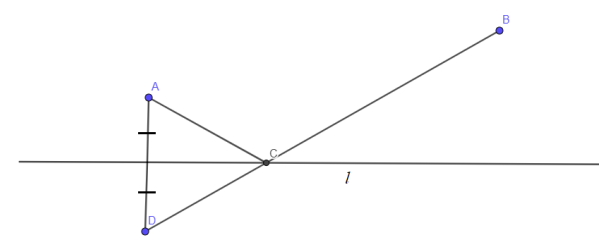
\includegraphics[width=1\textwidth]{graphics/Вспомогательная.png}
    Построим такую точку $D$, что она будет лежать симметрично $A$ относительно $l$. Тогда $BCD = BCA$. По неравенству треугольника, $BCD$ минимально, когда является прямой. Т. к. $\angle ACE = \angle DCE$ и, как было доказано $BD$ прямая, то $\angle (CA, l) = \angle (BC, l)$.


    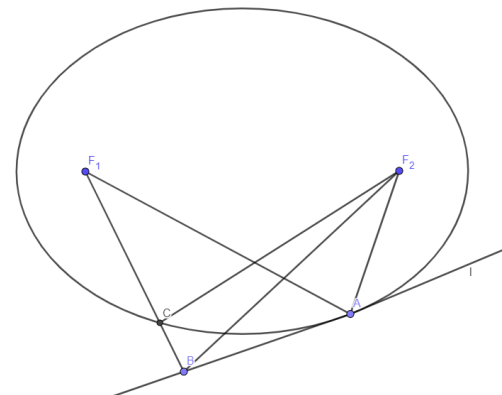
\includegraphics[width=0.6\textwidth]{graphics/Эллипс.png}

    Вернёмся к оптическому свойству. Для доказательства проведём касательную $l$ к эллипсу в точке $A$.
    Докажем, что через точку $A$ проходит кратчайший путь от $F_1$ до $F_2$ через $l$. Для этого возьмём точку $B \neq A$ на $l$.
    Тогда нужно доказать, что $F_1B + BF_2 > F_1A + AF_2$.

    Отметим на эллипсе точку $C$, лежащую на пересечении $F_1B$ с эллипсом. $F_1C + CF_2 = F_1A + AF_2$. При этом по неравенству треугольника $F_1C + CA_2 < F_1C + BC + BF_2 = F_1B + BF_2$. Следовательно, отрезки $F_1A$ и $F_2A$ образуют равные углы с прямой $l$, значит, по закону отражения, луч пройдёт через $F_2$.

    \section{Оптическое свойство гиперболы.}
    Оптическое свойство гиперболы заключается в том, что при выходе луча из одного фокуса, после его отражения при продлении луча в противоположную сторону он пройдёт через второй фокус.

    Для доказательства оптического свойства гиперболы пригодится решение вспомогательной задачи: Даны точки $A$ и $B$, лежащие по разные стороны от прямой $l$. Найти такую точку $C$, лежащую на $l$, что $|BC - AC|$ максимален.

    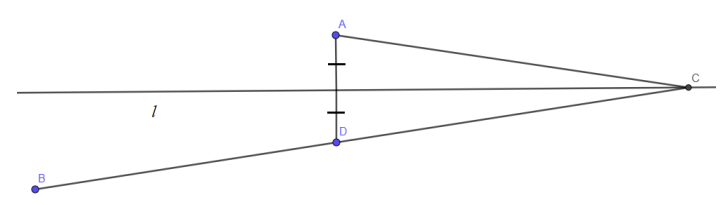
\includegraphics[width=0.8\textwidth]{graphics/Вспомогательная_гипербола.png}

    Возьмём точку $D$, симметричную $A$ относительно $l$. Тогда |BC - AC| = |BC - CD|. Тогда по неравенству треугольника максимум достигается в случае, если $D$ лежит на луче $BC$, т. к. тогда $AC = BC - BD \Rightarrow |BC - AC| = BD$. В иных случаях $AC > BC - BD \Rightarrow |BC - AC| < BD$.
    При этом углы между отрезками $AC$ и $BC$, и прямой $l$ равны.

    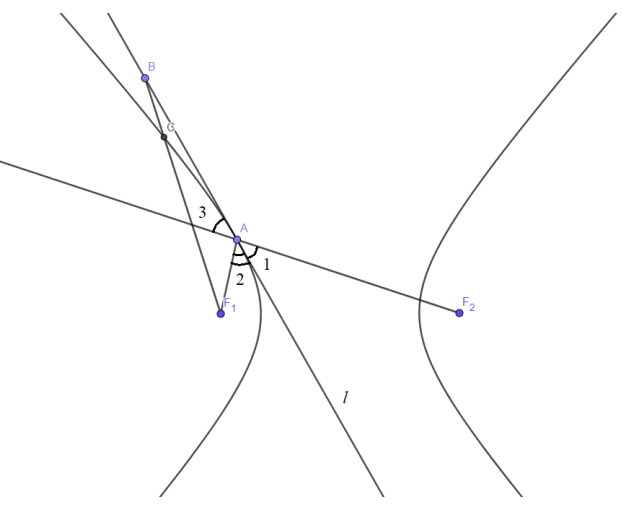
\includegraphics[width=0.8\textwidth]{graphics/Гипербола.png}

    Вернёмся к оптическому свойству гиперболы. Построим луч, выходящий из точки $F_1$ и касающийся гиперболы в точке $A$. Построим касательную к гиперболе в этой точке и назовём её $l$. Докажем, что отрезок $F_1A$ и луч $F_2A$ об разуют с прямой $l$ равные углы. Для этого достаточно доказать, что точка $A$ является решением вспомогательной задачи для точек $F_1$ и $F_2$ и прямой $l$.

    Для этого возьмём на прямой $l$ точку $B \neq A$ и докажем, что $|F_1A - F_2A| > |F_1B - F_2B|$. Для этого на пересечении $BF_1$ и гиперболы обозначим точку $C$. Так как мы ближе к $F_1$, чем к $F_2$, можно рассматривать неравенства $F_2A - F_1A > F_2B - F_1B$. При этом $F_2A - F_1A = F_2C - F_1C$. По неравенству треугольника очевидно, что $F_2C - F_1C < F_2B - F_1B \Rightarrow F_2A - F_1A < F_2B - F_1B$. Значит, угол 1 равен углу 2, угол 1 равен углу 3 т. к. они вертикальные $\Rightarrow$ угол 3 равен углу 2, следовательно, по закону отражения, продолжение луча в противоположную сторону проходит через точку $F_2$.


    \section{Оптическое свойство параболы.}
    Луч, выйдя из фокуса $F$ параболы, после отражения пойдёт перпендикулярно директрисе $l$.

    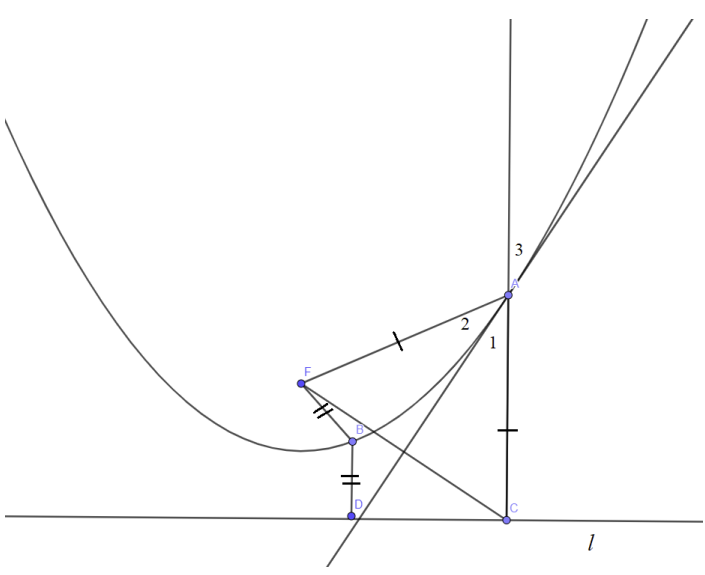
\includegraphics[width=0.8\textwidth]{graphics/Парабола.png}

    Обозначим за $A$ точку отражения луча от параболы, $C$ - проекцию этой точки на директрису. $B \neq A$ - произвольную точку на параболе, $D$ - проекцию точки $B$ на $l$. Сначала докажем, что вся парабола лежит слева от серединного перпендикуляра отрезка $FC$, т. е. он является касательной к параболе. Заметим, что $BC$ всегда больше $BD = BF$ по неравенству треугольника, если $B$ не совпадает с $C$. Отсюда $FC$ - касательная к параболе в точке $A$. Так как углы 1 и 2 находятся в равных треугольниках при равных сторонах, они равны. Углы 1 и 3 вертикальные, следовательно углы 2 и 3 тоже равны. Тогда после отражения луч пойдёт вертикально, то есть перпендикулярно директрисе.

    \section{Эллипс, гипербола и парабола как конические сечения.}
    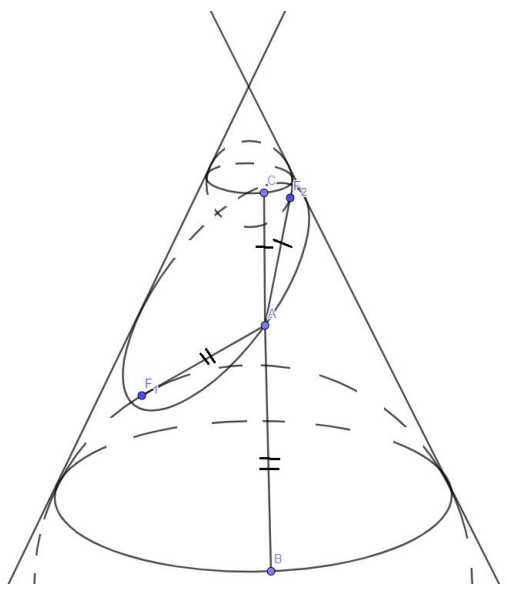
\includegraphics[width=0.8\textwidth]{graphics/Конус_эллипс.png}

    Длина касательных к одному шару равны. Отсюда, если взять сечение конуса, проходящее через его образующие, точку $A$ на его границе и два шара, касающихся конуса и сечения в точках $F_1, F_2$, а затем две точки ($B, C$) на окружностях, которыми эти сферы касаются конуса, то $AF_1 = AB$ и $AF_2 = AC$. Соответственно $AB + AC = \const \Rightarrow$ сечение конуса через образующие является эллипсом.

    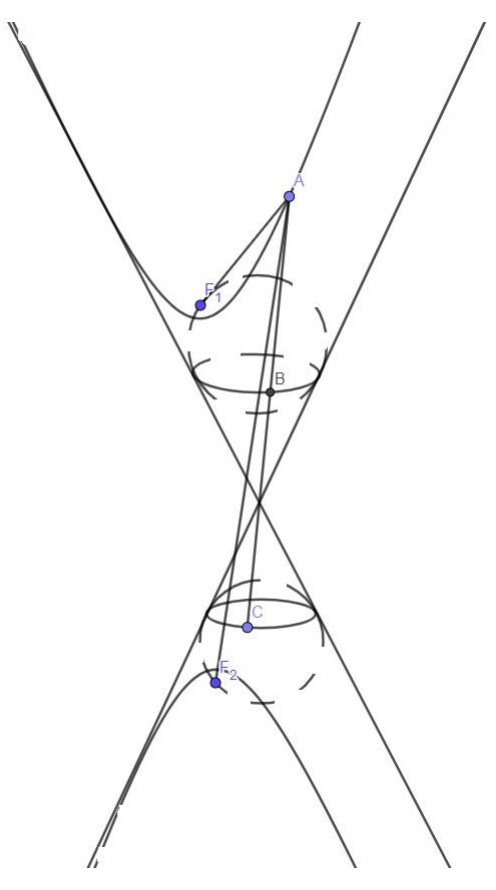
\includegraphics[width=0.4\textwidth]{graphics/Конус_гипербола.png}

    Возьмём сечение верхней и нижней полостей конуса, проходящее через их основания. Впишем два шара, касающихся конуса ($B, C$) и сечений ($F_1, F_2$) и точку $A$, находящуюся на границе плоскости сечения. По вышеописанным причинам $AF_1 = AB$, $AF_2 = AC$. Следовательно, $AF_2 - AF_1 = \const \Rightarrow$ сечение - гипербола.

    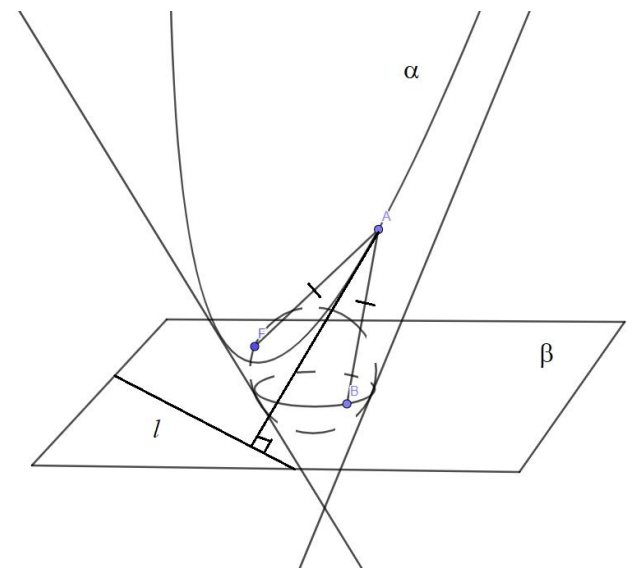
\includegraphics[width=0.8\textwidth]{graphics/Конус_парабола.png}

    Возьмём сечение плоскостью $\alpha$, параллельное одной из образующих конуса, шар, касающийся сечения в точке $F$ и касающийся конуса по окружности, точку $B$ на этой окружности, плоскость $\beta$, проходящую через эту окружность и прямую $l$ - пересечение $\alpha$ и $\beta$. Очевидно, что $AF = AB$ и $AB$ равно длине наклонной, направленной из точки $A$ к плоскости $\beta$ под тем же углом, что и образующие. Но расстояние от точки $A$ до прямой $l$ (обозначим проекцию $A$ на $l$ как $C$) тоже равно длине наклонной из $A$ к $\beta$. Отсюда $AF = AC \Rightarrow$ сечение является параболой, так как задаётся множеством точек равноудалённых от точки $F$ и прямой $l$.

    \section{Поверхности второго порядка. Определение, простейшие случаи.}
    Поверхностями второго порядка называют множества точек, являющихся корнями уравнения $ax^2 + by^2 + cz^2 + dxy + eyz + fxz + gx + hy + iz + j = 0$.

    Простейшие случаи:
    \begin{itemize}
        \item Точка ($x^2 + y^2 + z^2 = 0)$
        \item Прямая ($x^2 + y^2 = 0)$
        \item Плоскость ($x^2 = 0$)
        \item Две параллельных плоскости ($x^2 - 1 = 0$)
        \item Пустое множество ($x^2 + 1 = 0$)
    \end{itemize}

    Если выражение не зависит от $z$, поверхность называют цилиндром.

    Уравнение $x^2 + y^2 = z^2$ задаёт конус вращения.

    \section{Цилиндр (круговой, эллиптический, гиперболический, параболический), конус, эллипсоид: уравнения, свойства, эскизы.}
    Если выражение не зависит от $z$, то поверхность называют цилиндром (обычно рассматривают прямые цилиндры):
    \begin{itemize}
        \item $x^2 + y^2 = R^2$ - круговой цилиндр
        \item $\dfrac{x^2}{a^2} + \dfrac{y^2}{b^2} = 1$ - эллиптический цилиндр
        \item $\dfrac{x^2}{a^2} - \dfrac{y^2}{b^2} = 1$ - гиперболический цилиндр
        \item $y^2 = px$ - параболический цилиндр
    \end{itemize}

    Выражение вида $x^2 + y^2 = z^2$ задаёт прямой конус вращения. Можно представить два сечения - $z = \const$ - получим окружность - и $x = 0$ - получим две прямые $y = \pm z$. Таким образом можно представить прямой круговой конус как результат вращения двух прямых $y = \pm z$ вокруг оси $OZ$.

    Также можно представить конус как $\dfrac{x^2}{a^2} + \dfrac{y^2}{b^2} = \dfrac{z^2}{c^2}$, но это уже не будет конусом вращения.

    Эллипсоид задаётся выражением $\dfrac{x^2}{a^2} + \dfrac{y^2}{b^2} + \dfrac{z^2}{c^2} = 1$. Если рассмотреть сечение эллипсоида плоскостью, перпендикулярной одной из осей, то мы увидим эллипс. Эллипс можно представить как растянутый вдоль осей в $a, b, c$ раз шар с единичным радиусом. Тогда объём эллипсоида можно записать как объём единичного шара, умноженного на $abc$: $V = \dfrac{4}{3}\pi abc$.

    \section{Гиперболоид, однополостный и двуполостный: уравнения, свойства, эскизы.}
    Однополостным гиперболоидом называют поверхность, заданную выражением $x^2 + y^2 = z^2 + a^2$. При этом если взять его сечение в $x = a$, то мы увидим 2 прямые $y = \pm z$. Гиперболоид можно представить как результат вращения гиперболы вокруг не содержащей её прямой. Отсюда гиперболоид - это поверхность вращения и это верно для каждой точки в сечении $z = 0$ и это сечение будет представлять собой окружность.

    Иногда рассматривают гиперболоид вращения с дополнительными коэффициентами. Это означает, что гиперболоид растянули вдоль каждой из осей:
    \[
        \dfrac{x^2}{a^2} + \dfrac{y^2}{b^2} - \dfrac{z^2}{c^2} = 1
    \]

    $x^2 + y^2 = z^2 - a^2$ - двуполостный гиперболоид. Представляет собой результат вращения гиперболы вокруг содержащей её прямой. Состоит из двух несвязанных между собой частей. При растяжении вокруг осей получим:
    \[
        \dfrac{x^2}{a^2} + \dfrac{y^2}{b^2} - \dfrac{z^2}{c^2} = 1
    \]

    \section{Параболоид круговой, эллиптический и гиперболический: уравнения, свойства, эскизы.}


    \section{Вопросы к преподавателю}
    Какой смысл в поиске определителя матрицы при решении СЛАУ с параметром?

    Какие примеры можно привести к использованию центра масс для доказательства некоторых геометрических теорем?

    Что писать в пункте «применение метода координат для решения конструктивно-исследовательских задач по геометрии»? Исключительно примеры?

    \section{Найденные ошибки в лекциях}
    Лекция 04. Страница 5. Первый множитель третьего слагаемого определителя матрицы $3 \times 3$.

    Лекция 09. Страница 4. Третье алгебраическое свойство - $b$ не должно быть вектором.

    Лекция 11. Страница 7. Расстояние между скрещивающимися прямыми - "направляющих векторов плоскости".

    Лекция 13. Страница 2. Вывод уравнения параболы - "а уравнение директрисы y = -1".

    Лекция 13. Страница 7. Оптическое свойство гиперболы - "Пусть С – точка пересечения эллипса".

    Лекция 13. Страница 9. Эллипс, гипербола и парабола как конические сечения - "наклонное сечение прямого кругового цилиндра является конусом".

    Лекция 13. Страница 11. Как мне кажется, там ошибка в рисунке.
\end{sloppypar}
\end{document}
